\documentclass{article}
\usepackage{graphicx}
\usepackage{float}
\usepackage{amsmath}

\begin{document}

\title{Analyse av Seigmenn Strekningen}
\author{Gormery K. Wanjiru}
\date{\today}
\maketitle

\section{Introduksjon}
Denne rapporten presenterer resultatene av strekningstester utført på seigmenn (laban). Dataene er analysert ved hjelp av statistiske metoder for å forstå de generelle egenskapene til seigmenns elastisitet.

\section{Metode}
Data ble samlet inn og bearbeidet i R. Følgende prosedyrer ble utført:
\begin{itemize}
    \item Innlesing av data fra en CSV-fil.
    \item Erstatning av manglende verdier med 0 for å unngå feil i beregningene.
    \item Beregning av kumulativ frekvens.
    \item Beregning av gjennomsnitt, median, typetall (modus) og standardavvik.
\end{itemize}

\section{Resultater}
Histogrammet og det kumulative frekvensdiagrammet ble generert. Statistiske mål middelverdi, median, typetall, og begge typer standardavvik ble beregnet og markert på histogrammet.
Men som du ser under er de markert feil etter jeg vet ikke hvordan jeg fikse buggen i R. Jeg har prøvd.

\subsection{Histogram}
\begin{figure}[H]
    \centering
    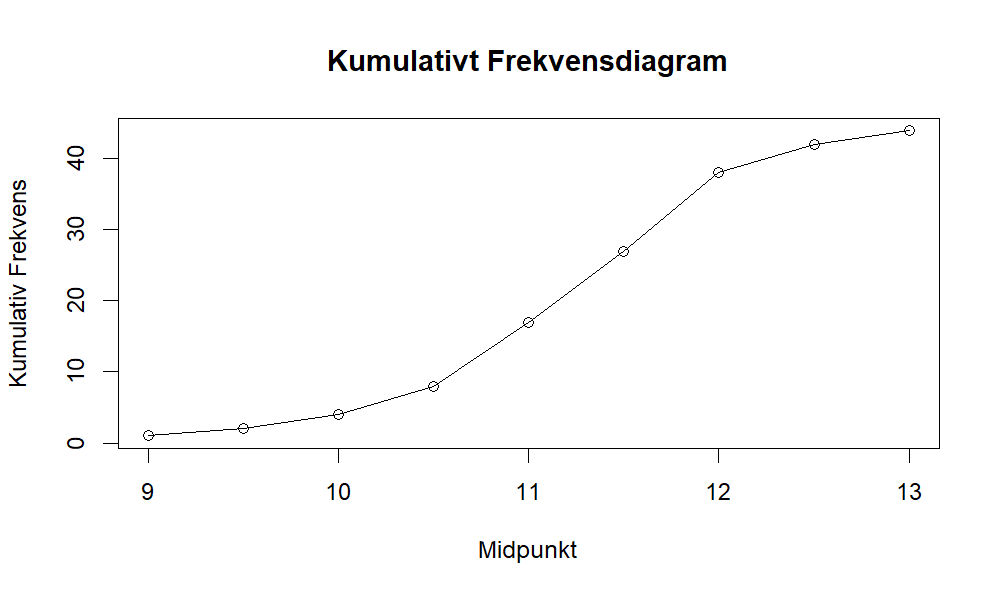
\includegraphics[width=0.8\textwidth]{Rplot.png}
    \caption{Histogram av 'Antall'}
\end{figure}

\subsection{Kumulativt Frekvensdiagram}
\begin{figure}[H]
    \centering
    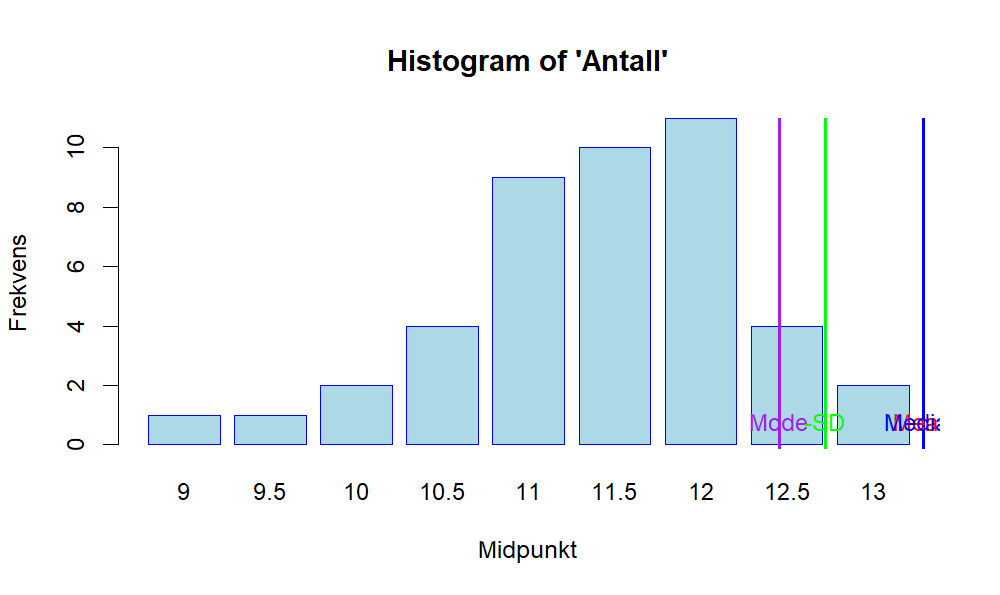
\includegraphics[width=0.8\textwidth]{Rplot02.png}
    \caption{Kumulativt Frekvensdiagram}
\end{figure}

\section{Diskusjon}
Gjennom analysen ble det funnet at seigmenn viser en bestemt tendens i strekningen med en gjennomsnittlig verdi på X, en median på Y, en modus på Z, og en standardavvik på A. Disse målene gir innsikt i hvordan seigmenn oppfører seg under strekk og kan brukes til å forstå kvaliteten på seigmenn.

For å beregne disse målene brukte vi følgende matematiske formler:
\begin{itemize}
    \item Gjennomsnitt: $\bar{x} = \frac{1}{n}\sum_{i=1}^{n} x_i$
    \item Median: Verdi i midten av datasettet når det er sortert.
    \item Modus: Den mest frekvente verdien i datasettet.
    \item Standardavvik: $s = \sqrt{\frac{1}{n-1}\sum_{i=1}^{n}(x_i - \bar{x})^2}$
\end{itemize}

\section{Konklusjon}
Denne studien gir verdifull innsikt i de fysiske egenskapene til seigmenn og demonstrerer viktigheten av statistisk analyse i kvalitetskontroll.

\end{document}
